\chapter{Red Black Tree Data Structure}
A red-black tree is a special type of binary search tree with one extra bit of storage per node, its color which can be either red or black. Also, we keep the tree approximately balanced by enforcing some properties on the tree.
\begin{definition}{Perfect Binary Tree}{}
	It is a Binary Tree in which every internal node has exactly two children and all leaves are at the same level.
\end{definition}
\begin{Lemma}{}{}
	Every perfect binary tree with $k$ leaves has $2k-1$  nodes (i.e. $k-1$ internal nodes).
\end{Lemma}
\begin{definition}{Red Black Tree}{}
	\begin{minipage}{0.5\textwidth}
		A red-black tree is a binary tree with the following properties:
		\begin{itemize}
			\item Every internal node is key/NIL node. Every leaf is a ``NIL'' node.
			\item Each node (NIL and key) is colored either red or black.
			\item  Root and NIL nodes are always black.
			\item Any child of a red node is black.
			\item The path from root to any leaf has the same number of black nodes.
		\end{itemize}
	\end{minipage}\hfill
	\begin{minipage}{0.49\textwidth}
		\centering
		\usetikzlibrary{trees,arrows,positioning, calc}
		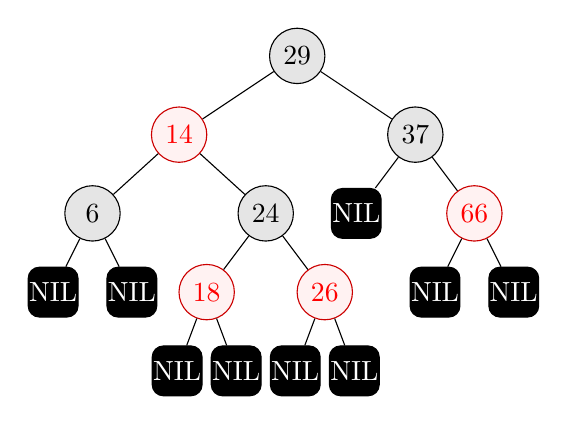
\begin{tikzpicture}[
				level/.style={sibling distance=30mm/#1},
				level distance=10mm,
				redVertex/.style={draw=red!80!black,fill=red!5!white,circle,minimum size=20pt,inner sep=0pt, text=red},
				blackVertex/.style={draw,fill=black!10!white,   circle,minimum size=20pt,inner sep=0pt},
				nil/.style={draw,fill=black,rectangle,rounded corners, minimum size=18pt,inner sep=0pt, text=white}]
			\node [blackVertex] (r){29}
			child {
					node[redVertex] {14}
					child [sibling distance=22mm] {
							node[blackVertex] {6}
							child {node [nil] {NIL}}
							child {node [nil] {NIL}}
						}
					child [sibling distance=22mm] {
							node [blackVertex] {24}
							child [sibling distance=15mm] {
									node [redVertex] {18}
									child {node [nil] {NIL}}
									child {node [nil] {NIL}}
								}
							child [sibling distance=15mm] {
									node [redVertex] {26}
									child {node [nil] {NIL}}
									child {node [nil] {NIL}}
								}
						}
				}
			child {
					node[blackVertex] {37}
					child {node [nil] {NIL}}
					child {
							node [redVertex] {66}
							child {node [nil] {NIL}}
							child { node [nil] {NIL}}
						}
				};
		\end{tikzpicture}
		\captionof{figure}{A Red Black Tree}
		\label{fig:red-black-tree}
	\end{minipage}
\end{definition}

We call the number of black nodes on any simple path from  but not including a node $x$ down to a leaf the \emph{black-height} of the node, denoted by $bh(x)$. We generally confine our interest to the internal nodes of a red-black tree, since they hold the key values.
\begin{Lemma}{}{}
	A Red-Black Tree with $n$ internal nodes or key nodes has height at most $O(\log n)$.
\end{Lemma}
\begin{proof}
	We will first show that for any subtree rooted at node $x$ contains at least $2^{bh(x)}-1$ internal nodes. We will show this using induction on the height of the tree. For the base case let height of $x$ is $0$. Then $x$ must be a leaf. Therefore, the subtree rooted at $x$ has at least $bh(x)=0$. Hence, $2^{bh(x)}-1=2^0-1=0$  nodes which is true. For inductive step let $x$ has some positive height, and it is an internal node of the R-B Tree. Now $x$ has two children. Hence, each child has black-height either $bh(x)$ or $bh(x)-1$. By inductive hypothesis, the subtrees rooted at the children of $x$ have at least $2^{bh(x)-1}-1$ internal nodes. Thus, subtree rooted at $x$ has at least $2^{bh(x)-1}-1+2^{bh(x)-1}-1+1=2^{bh(x)}-1$ internal nodes.

	Now if the R-B tree has height $h$. Then any path from the root to a leaf at least half the nodes including the root must be black. So $bh(\emph{root})\geq \frac{h}2$. Thus, $n\geq 2^{\frac{h}2}-1\implies h\leq 2\log(n+1)$. Hence, we have the lemma.
\end{proof}
\nt{
	\begin{minipage}{0.3\textwidth}
		\centering
		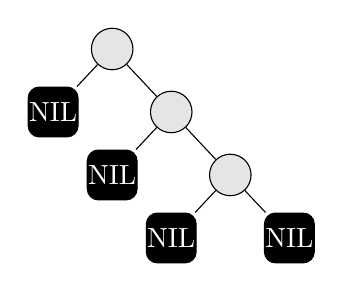
\begin{tikzpicture}[
				level distance=8mm,
				vertex/.style={draw,fill=black!10!white,circle,minimum size=15pt,inner sep=0pt},
				nil/.style={draw,fill=black,rectangle,rounded corners, minimum size=18pt,inner sep=0pt, text=white}
			]
			\node[vertex] (a) {}
			child { node [nil] {NIL} }
			child {
					node [vertex] (b) {}
					child { node [nil] {NIL} }
					child {
							node [vertex] (c) {}
							child { node [nil] {NIL} }
							child { node [nil] {NIL} }
						}
				};
		\end{tikzpicture}
	\end{minipage}\hfill
	\begin{minipage}{0.69\textwidth}
		Not all trees can be colored in a way that satisfies the properties of a red-black tree. Consider the following tree:\parinn

		In this example the root has to be black. The other two internal nodes can not be black since otherwise the path from the leaf of the root to root has only 2 black nodes but in the path from bottom most leaf to root will have 3. Then those two internal nodes has to be red. But that violates the property that a red node can not have a red child. Hence, this tree can not be colored in a way that satisfies the properties of a red-black tree.
	\end{minipage}
}

Since by the lemma the R-B tree has height at most $O(\log n)$ and it is a binary search tree we can perform search of a node using \textsc{Find} in $O(\log n)$ time. So now we will focus on the insertion and deletion operations in a red-black tree.  To insert or delete a node in a red-black tree we will  rotations to balance the tree again. So first we will visit rotations.
\section{Rotation}
A rotation is a local operation that changes the structure of a binary tree without violating the binary search tree property. There are two types of rotations: left rotation and right rotation.

When we do a left rotation on a node we assume that its right child is not NIL. The left rotation ``pivots'' around the link from the node to its right child and makes the right child the new root of the subtree with the ode as its left child.  Similarly, we can explain the right rotation. The rotations behave like the following:

\begin{figure}[!h]
	\centering
	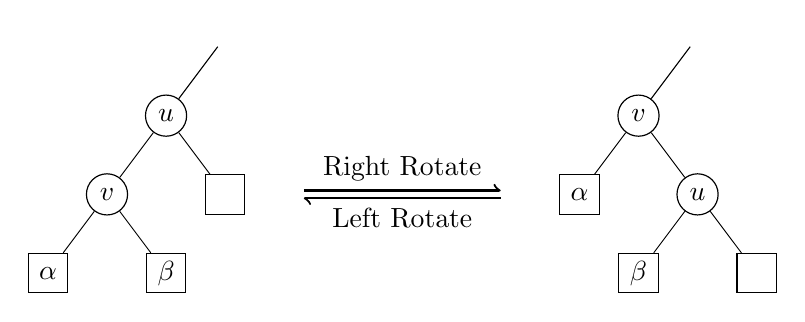
\begin{tikzpicture}[
			every node/.style={align=center, line width=0.15mm},
			level 1/.style={level distance=1cm, sibling distance=1.5cm},  % Adjusted distance for level 1
			level 2/.style={sibling distance=1.5cm},   % Adjusted distance for level 2
			square/.style={draw, shape=rectangle, minimum width=0.5cm, minimum height=0.5cm, inner sep=0pt, text width=0.5cm, text centered},
			circle/.style={draw, shape=circle, minimum width=0.5cm, minimum height=0.5cm, inner sep=0pt, text width=0.5cm, text centered},
			filled/.style={fill=white, , draw, line width=0.12mm},  % Style for filled nodes
			every edge/.style = {draw, latex'-latex' , line width=0.3mm, dotted,},
			parentarrow/.style={line width=0.12mm},  % Style for arrows from nodes to children
		]

		% Leftmost tree
		\node (A0) {}
		child{
				node[circle] (A1) {$u$}
				child {node[circle] (B1) {$v$}
						child {node[square] (D1) {$\alpha$} edge from parent[parentarrow]}
						child {node[square] (E1) {$\beta$} }
						edge from parent[parentarrow]
					}
				child {node[square,filled] (C1) {$\gm$} edge from parent[parentarrow]}
			}
		child [missing] { node (A5) {} };

		% Right tree
		\begin{scope}[shift={(6,0)}]
			\node (AA0) {}
			child{
					node[circle] (A2) {$v$}
					child {node[square,filled] (C2) {$\alpha$} edge from parent[parentarrow]}
					child {node[circle] (B2) {$u$}
							child {node[square] (D2) {$\beta$} edge from parent[parentarrow]}
							child {node[square] (E2) {$\gm$} }
							edge from parent[parentarrow]
						}
				}
			child [missing] { node (AA5) {} };

		\end{scope}

		\draw[thick, -left to] ($(C1)+(1,0.05)$) -- node[midway, above] {Right Rotate} ($(C2)+(-1,0.05)$);
		\draw[thick, -left to] ($(C2)+(-1,-0.05)$) -- node[midway, below] {Left Rotate}($(C1)+(1,-0.05)$)  ;
	\end{tikzpicture}
	\caption{Left and Right rotate about $u-v$}
\end{figure}\parinf

\begin{minipage}{0.46\textwidth}
	\begin{algorithm}[H]
		\caption{\textsc{Left-Rotate}$({T,x})$}
		\DontPrintSemicolon
		$y\longleftarrow x.\emph{right}$\;
		$x.\emph{right}\longleftarrow y.\emph{left}$\;
		\If{$y.\emph{left}\neq \emph{NIL}$}{
			$y.\emph{left}.\emph{parent}\longleftarrow x$\;
		}
		$y.\emph{parent}\longleftarrow x.\emph{parent}$\;
		\If{$x.\emph{parent}==\emph{NIL}$}{
			$T.\emph{root}\longleftarrow y$\;
		}
		\ElseIf{$x== x.\emph{parent}.\emph{left}$}{
			$x.\emph{parent}.\emph{left}\longleftarrow y$\;
		}
		\Else{
			$x.\emph{parent}.\emph{right}\longleftarrow y$\;
		}
		$y.\emph{left}\longleftarrow x$\;
		$x.\emph{parent}\longleftarrow y$
	\end{algorithm}
\end{minipage}\hfill
\begin{minipage}{0.46\textwidth}
	\begin{algorithm}[H]
		\caption{\textsc{Right-Rotate}$({T,x})$}
		\DontPrintSemicolon
		$y\longleftarrow x.\emph{left}$\;
		$x.\emph{left}\longleftarrow y.\emph{right}$\;
		\If{$y.\emph{right}\neq \emph{NIL}$}{
			$y.\emph{right}.\emph{parent}\longleftarrow x$\;
		}
		$y.\emph{parent}\longleftarrow x.\emph{parent}$\;
		\If{$x.\emph{parent}==\emph{NIL}$}{
			$T.\emph{root}\longleftarrow y$\;
		}
		\ElseIf{$x== x.\emph{parent}.\emph{left}$}{
			$x.\emph{parent}.\emph{left}\longleftarrow y$\;
		}
		\Else{
			$x.\emph{parent}.\emph{right}\longleftarrow y$\;
		}
		$y.\emph{right}\longleftarrow x$\;
		$x.\emph{parent}\longleftarrow y$
	\end{algorithm}
\end{minipage}\parinn

Both \textsc{Left-Rotate} and \textsc{Right-Rotate} take $O(1)$ time. Only some constantly many pointers are changed by rotation all other attributes in a node remain the same.
\section{Insertion}
We will now describe how to insert a node in a red-black tree in $O(\log n)$ time. We will insert the node in the tree in place of a leaf replacing a NIL node. After that we will color the node red. Let the node added is $v$. We define the attribute \emph{uncle} which is basically sibling of the parent. Now two cases can happen:
\begin{enumerate}[label=Case \Roman*:, leftmargin=*]
	\item $v.\emph{uncle}.color=$ Red: Then $v.\emph{parent}.\emph{parent}$  is black. In this case we can recolor $v.\emph{parent}.\emph{parent}$ to red and both $v.\emph{parent}$ and $v.\emph{uncle}$ to be black. This will preserve the number of black nodes in any simple path from root to any leaf.
	      \begin{figure}[!h]
		      \centering
		      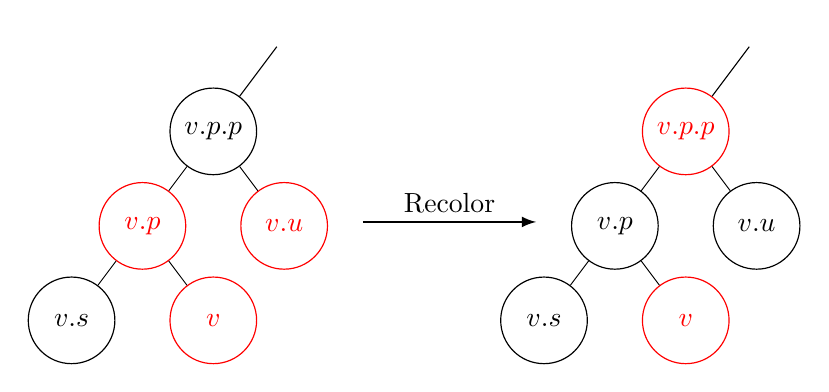
\begin{tikzpicture}[
				      every node/.style={align=center, line width=0.15mm},
				      level 1/.style={level distance=1.2cm, sibling distance=1.8cm},  % Adjusted distance for level 1
				      level 2/.style={sibling distance=1.8cm},   % Adjusted distance for level 2
				      redVertex/.style={draw, shape=circle, minimum width=1.1cm, minimum height=0.5cm, inner sep=0pt, text width=1cm, text centered, text=red!75!black, color=red},
				      blackVertex/.style={draw, shape=circle, minimum width=1.1cm, minimum height=0.5cm, inner sep=0pt, text width=1cm, text centered},
				      every edge/.style = {draw, latex'-latex' , line width=0.3mm, dotted,},
				      Rparentarrow/.style={line width=0.12mm, color=red},  % Style for arrows from nodes to children
				      parentarrow/.style={line width=0.12mm}
			      ]

			      % Leftmost tree
			      \node (AA0) {}
			      child{
					      node[blackVertex] (A2) {$v.p.p$}
					      child {node[redVertex] (B2) {$v.p$}
							      child {node[blackVertex] (D2) {$v.s$} edge from parent[parentarrow]}
							      child {node[redVertex] (E2) {$v$} }
							      edge from parent[parentarrow]
						      }
					      child {node[redVertex] (C2) {$v.u$} edge from parent[parentarrow]}
				      }
			      child [missing] { node (AA5) {} };
			      % Right tree
			      \begin{scope}[shift={(6,0)}]
				      \node (A0) {}
				      child{
						      node[redVertex] (A1) {$v.p.p$}
						      child {node[blackVertex] (B1) {$v.p$}
								      child {node[blackVertex] (D1) {$v.s$} edge from parent[parentarrow]}
								      child {node[redVertex] (E1) {$v$} }
								      edge from parent[parentarrow]
							      }
						      child {node[blackVertex] (C1) {$v.u$} edge from parent[parentarrow]}
					      }
				      child [missing] { node (A5) {} };
			      \end{scope}

			      \draw[thick, -latex] ($(C2)+(1,0.05)$) -- node[midway, above] {Recolor} ($(B1)+(-1,0.05)$);
		      \end{tikzpicture}
	      \end{figure}
	      Now the color of $v.\emph{parent}.\emph{parent}$ is red, and therefore we iterate the same process on $v.\emph{parent}.\emph{parent}$.
	\item $v.\emph{uncle}.\emph{color}=$ Black: In this case we need two rotations. First we do a left rotation on $v.\emph{parent}$. After that we do a right rotation on $v.\emph{parent}.\emph{parent}$. After the rotations, we recolor the nodes.
	      \begin{figure}[!h]
		      \centering
		      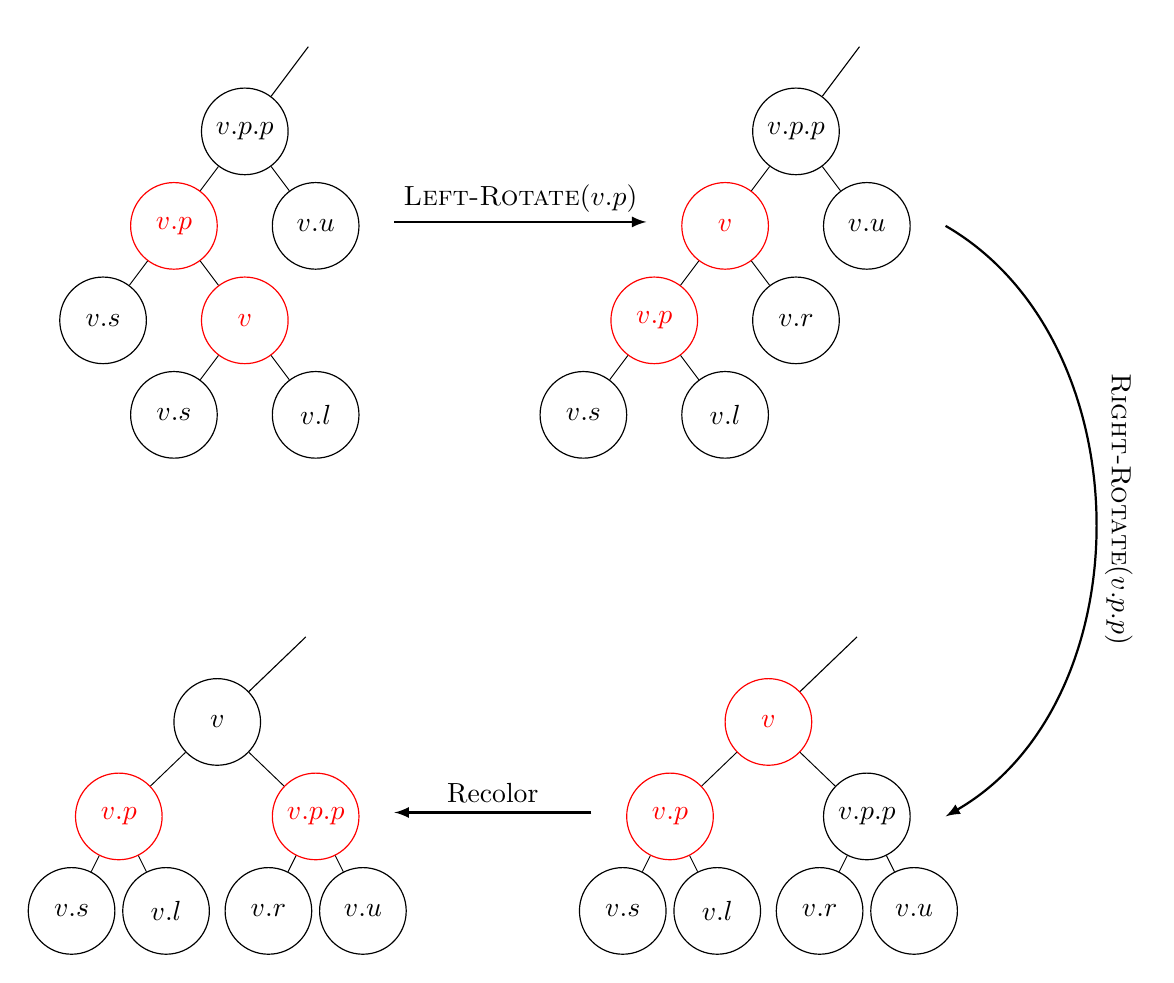
\begin{tikzpicture}[
				      every node/.style={align=center, line width=0.15mm},
				      level 1/.style={level distance=1.2cm, sibling distance=1.8cm},  % Adjusted distance for level 1
				      level 2/.style={sibling distance=1.8cm},   % Adjusted distance for level 2
				      redVertex/.style={draw, shape=circle, minimum width=1.1cm, minimum height=0.5cm, inner sep=0pt, text width=1cm, text centered, text=red!75!black, color=red},
				      blackVertex/.style={draw, shape=circle, minimum width=1.1cm, minimum height=0.5cm, inner sep=0pt, text width=1cm, text centered},
				      every edge/.style = {draw, latex'-latex' , line width=1mm},
				      Rparentarrow/.style={line width=0.12mm, color=red},  % Style for arrows from nodes to children
				      parentarrow/.style={line width=0.12mm}
			      ]

			      % Leftmost tree
			      \begin{scope}[shift={(1,0)}]
				      \node (AA0) {}
				      child{
						      node[blackVertex] (A2) {$v.p.p$}
						      child {node[redVertex] (B2) {$v.p$}
								      child {node[blackVertex] (D2) {$v.s$} edge from parent[parentarrow]}
								      child {
										      node[redVertex] (E2) {$v$}
										      child { node[blackVertex] (F1) {$v.s$} edge from parent[parentarrow] }
										      child { node[blackVertex] (G1) {$v.l$} edge from parent[parentarrow] }
									      }
								      edge from parent[parentarrow]
							      }
						      child {node[blackVertex] (C2) {$v.u$} edge from parent[parentarrow]}
					      }
				      child [missing] { node (AA5) {} };
			      \end{scope}
			      % Right tree
			      \begin{scope}[shift={(8,0)}]
				      \node (A0) {}
				      child{
						      node[blackVertex] (A1) {$v.p.p$}
						      child {node[redVertex] (B1) {$v$}
								      child {
										      node[redVertex] (D1) {$v.p$} edge from parent[parentarrow]
										      child { node[blackVertex] (F1) {$v.s$} edge from parent[parentarrow] }
										      child { node[blackVertex] (G1) {$v.l$} edge from parent[parentarrow] }
									      }
								      child {node[blackVertex] (E1) {$v.r$} }
								      edge from parent[parentarrow]
							      }
						      child {node[blackVertex] (C1) {$v.u$} edge from parent[parentarrow]}
					      }
				      child [missing] { node (A5) {} };
			      \end{scope}
			      \begin{scope}[shift={(8,-7.5)}]
				      \node (AAA0) {}
				      child[sibling distance=2.5cm]{
						      node[redVertex] (A3) {$v$}
						      child[sibling distance=2.5cm] {node[redVertex] (B3) {$v.p$}
								      child[sibling distance=1.2cm] {node[blackVertex] (D3) {$v.s$} edge from parent[parentarrow]}
								      child[sibling distance=1.2cm] {node[blackVertex] (E3) {$v.l$} }
								      edge from parent[parentarrow]
							      }
						      child[sibling distance=2.5cm] {
								      node[blackVertex] (C3) {$v.p.p$} edge from parent[parentarrow]
								      child[sibling distance=1.2cm] { node[blackVertex] (F3) {$v.r$} edge from parent[parentarrow] }
								      child[sibling distance=1.2cm] { node[blackVertex] (G3) {$v.u$} edge from parent[parentarrow] }
							      }
					      }
				      child [sibling distance=2.5cm,missing] { node (AAA5) {} };
			      \end{scope}
			      \begin{scope}[shift={(1,-7.5)}]
				      \node (AAAA0) {}
				      child[sibling distance=2.5cm]{
						      node[blackVertex] (A4) {$v$}
						      child[sibling distance=2.5cm] {node[redVertex] (B4) {$v.p$}
								      child[sibling distance=1.2cm] {node[blackVertex] (D4) {$v.s$} edge from parent[parentarrow]}
								      child[sibling distance=1.2cm] {node[blackVertex] (E4) {$v.l$} }
								      edge from parent[parentarrow]
							      }
						      child[sibling distance=2.5cm] {
								      node[redVertex] (C4) {$v.p.p$} edge from parent[parentarrow]
								      child[sibling distance=1.2cm] { node[blackVertex] (F4) {$v.r$} edge from parent[parentarrow] }
								      child[sibling distance=1.2cm] { node[blackVertex] (G4) {$v.u$} edge from parent[parentarrow] }
							      }
					      }
				      child [sibling distance=2.5cm,missing] { node (AAAA5) {} };
			      \end{scope}
			      \draw[thick, -latex] ($(C2)+(1,0.05)$) -- node[midway, above] {\textsc{Left-Rotate}$(v.p)$} ($(B1)+(-1,0.05)$);
			      \draw($(C1)+(1,0)$) edge [bend left=60, thick, -latex]  node[midway, right, rotate=-90, xshift=-2cm, yshift=0.3cm] {\textsc{Right-Rotate}$(v.p.p)$} ($(C3)+(1,0)$);
			      \draw[thick, -latex] ($(B3)+(-1,0.05)$) -- node[midway, above] {Recolor} ($(C4)+(1,0.05)$);
		      \end{tikzpicture}
	      \end{figure}
	      The color of $v.\emph{parent}.\emph{parent}$ will be black and the color of $v.\emph{parent}$ will be red. The color of $v$ will remain red. This will preserve the number of black nodes in any simple path from root to any leaf. And this case now stabilizes the tree, and we can stop the process.
\end{enumerate}
So analyzing the insertion process we can insert a node in a red-black tree and using the two cases we can recolor the nodes the balance the tree.\parinf

\begin{minipage}{0.46\textwidth}
	\begin{algorithm}[H]
		\caption{\textsc{RB-Insert}$(T,v)$}
		\DontPrintSemicolon
		$y\longleftarrow \emph{NIL}$, $x\longleftarrow T.\emph{root}$\;
		\While{$x\neq \emph{NIL}$}{
			$y\longleftarrow x$\;
			\If{$v.\emph{key}<x.\emph{key}$}{
				$x\longleftarrow x.\emph{left}$\;
			}
			\Else{
				$x\longleftarrow x.\emph{right}$\;
			}
		}
		$v.\emph{parent}\longleftarrow y$\;
		\If{$y==\emph{NIL}$}{
			$T.\emph{root}\longleftarrow v$\;
		}
		\ElseIf{$v.\emph{key}<y.\emph{key}$}{
			$y.\emph{left}\longleftarrow v$\;
		}
		\Else{
			$y.\emph{right}\longleftarrow v$\;
		}
		$v.\emph{left}\longleftarrow \emph{NIL}$,
		$v.\emph{right}\longleftarrow \emph{NIL}$, $v.\emph{color}\longleftarrow RED$\;
		\textsc{RB-Insert-Fixup}$(T,v)$\;
	\end{algorithm}
\end{minipage}\hfill
\begin{minipage}{0.5\textwidth}
	\begin{algorithm}[H]
		\SetKwComment{Comment}{// }{}
		\caption{\textsc{RB-Insert-Fixup}$(T,v)$}
		\DontPrintSemicolon
		\While{$v.\emph{parent}.\emph{color}==RED$}{
			\If{$v.\emph{parent}.\emph{parent}==NIL$}{$v.\emph{parent}.\emph{color}\longleftarrow BLACK$\;Break\;}
			$vu\longleftarrow v.\emph{parent}.\emph{parent}.\emph{right}$\Comment*{Uncle}
			$vpp\longleftarrow v.\emph{parent}.\emph{parent}$\;
			\If{$vu.\emph{color}==RED$}{
				$v.\emph{parent}.\emph{color}\longleftarrow BLACK$\Comment*{Case I}
				$vu.\emph{color}\longleftarrow BLACK$\;
				$vpp.\emph{color}\longleftarrow RED$\;
				$v\longleftarrow vpp$
			}
			\Else{
				\textsc{Left-Rotate}$(T,v.\emph{parent})$\Comment*{Case II}
				\textsc{Right-Rotate}$(T,vpp)$\;
				$v.\emph{color}\longleftarrow BLACK$\;
				$vpp.\emph{color}\longleftarrow RED$\;
				Break
			}
		}
	\end{algorithm}
\end{minipage}
\parinn

Since the case I can happen at most $O(\log n)$ times as each use of case I increase the height by $2$ the while loop can run at most $O(\log n)$ times. Therefore, insertion of a node in a red-black tree takes $O(\log n)$ time.
\section{Deletion}
Like insertion, deletion of a node involves recoloring and rotations to maintain the properties of a red-black tree. Here we will use a notion of double-black color. In the deletion we will use something called in-order traversal of the binary tree and use successor and predecessor of a node in the traversal. \begin{Definition}{In-Order Traversal}{}
	In-Order Traversal of a binary tree is a traversal where:\begin{itemize}
		\item Recursively traverse the current node left subtree.
		\item Visit the current node.
		\item Recursively traverse the current node right subtree.
	\end{itemize}
	The in-order \emph{successor} (\emph{predecessor}) of a node is the next (previous) node in the in-order traversal of the tree.
\end{Definition}
\begin{observation}
	For any node $x$ the in-order successor of $x$ is the leftmost node in the right subtree of $x$. Similarly, the in-order predecessor of $x$ is the rightmost node in the left subtree of $x$.
\end{observation}
To delete a node $x$ we will replace its \emph{key} by the key of its in-order successor or predecessor (say $y$) and then delete $y$ i.e. after replacing the key of $x$ by the key of $y$, it will still have the color of $x.\emph{color}$. We replace with in-order successor unless $x$ has no right child. In that case we replace with in-order predecessor. If $x$ has no children then we have $y=x$.
\nt{$y$ is either a non-NIL leaf or has exactly one child.}

\begin{enumerate}
	\item $y$ has a child then child must be colored red since otherwise the NIL child of $y$ and any NIL node in the subtree rooted at child of $y$ will have different black-height. Therefore, $y$ must be colored black. Hence, we replace $y$ by its child and color it black.
	\item $y$ is a non-NIL leaf and its colored red. Then we can simply remove $y$ from the tree.
\end{enumerate}
So the only case remained to analyze is when $y$ is a non-NIL leaf and colored black. Now the situation is complicated since removing $y$ would create black-height imbalance in the tree.
\begin{observation}
	If $y.\emph{color}$ is black then $y$ must have a sibling since otherwise sibling of $y$ is NIL. Then that NIL node and any NIL node in the subtree rooted at $y$ will have different black-height.
\end{observation}
So we replace $y$ with a NIL node and color it \emph{double-black} which  will be counted has $2$ black nodes to maintain the black-height. Now we will resolve the double-black color by rotation, recoloring or pushing up the double-black color. Now we will use the following pointers \begin{itemize}
	\item $y.\emph{sibling}$ to denote the sibling of $y$.
	\item $y.\emph{left-nephew}$ and  $y.\emph{right-nephew}$ to denote the left and right child of $y.\emph{sibling}$.
\end{itemize} We will use the following cases to resolve the double-black color:
\begin{enumerate}[label=Case \Roman*:, leftmargin=*]
	\item  $y.\emph{sibling},y.\emph{parent},y.\emph{left-nephew},y.\emph{right-nephew}$ are Black. In this case we can move the double black node to the parent of $y$ and recolor the $y$ has black node and sibling of $y$ red color.
	      \begin{figure}[!h]
		      \centering
		      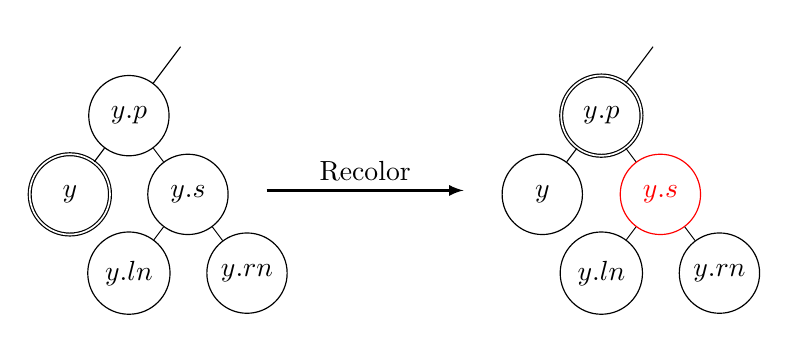
\begin{tikzpicture}[level distance=1cm,
				      every node/.style={align=center, line width=0.15mm},
				      level 1/.style={sibling distance=1.5cm},
				      level 2/.style={sibling distance=1.5cm},
				      redVertex/.style={
						      draw, shape=circle,
						      minimum width=0.9cm, minimum height=0.5cm,
						      inner sep=0pt, text width=1cm, text centered,
						      text=red!75!black, color=red
					      },
				      blackVertex/.style={
						      draw, shape=circle,
						      minimum width=0.9cm, minimum height=0.5cm,
						      inner sep=0pt, text width=1cm, text centered
					      },
				      doubleBlackVertex/.style={
						      draw, double, shape=circle,
						      minimum width=0.9cm, minimum height=0.5cm,
						      inner sep=0pt, text width=1cm, text centered
					      },
				      every edge/.style = {draw, latex'-latex', line width=0.3mm, dotted},
				      parentarrow/.style={line width=0.12mm}
			      ]

			      % Leftmost tree
			      \node (AA0) {}
			      child{
					      node[blackVertex] (A2) {$y.p$}
					      child {node[doubleBlackVertex] (B2) {$y$}}
					      child {
							      node[blackVertex] (C2) {$y.s$} edge from parent[parentarrow]
							      child {node[blackVertex] (D2) {$y.ln$} edge from parent[parentarrow]}
							      child {node[blackVertex] (E2) {$y.rn$} }
							      edge from parent[parentarrow]
						      }
				      }
			      child [missing] { node (AA5) {} };
			      % Right tree
			      \begin{scope}[shift={(6,0)}]
				      \node (A0) {}
				      child{
						      node[doubleBlackVertex] (A1) {$y.p$}
						      child {node[blackVertex] (B1) {$y$}}
						      child {
								      node[redVertex] (C1) {$y.s$} edge from parent[parentarrow]
								      child {node[blackVertex] (D1) {$y.ln$} edge from parent[parentarrow]}
								      child {node[blackVertex] (E1) {$y.rn$} }
								      edge from parent[parentarrow]
							      }
					      }
				      child [missing] { node (A5) {} };
			      \end{scope}

			      \draw[thick, -latex] ($(C2)+(1,0.05)$) -- node[midway, above] {Recolor} ($(B1)+(-1,0.05)$);
		      \end{tikzpicture}
	      \end{figure}
	\item $y.\emph{sibling},y.\emph{left-nephew},y.\emph{right-nephew}$ are Black \& $y.\emph{parent}$ is Red. Here we recolor $y.\emph{parent}$ to black and $y.\emph{sibling}$ to red. This will preserve the number of black nodes in any  path from root to any leaf. So we stop.\begin{figure}[!h]
		      \centering
		      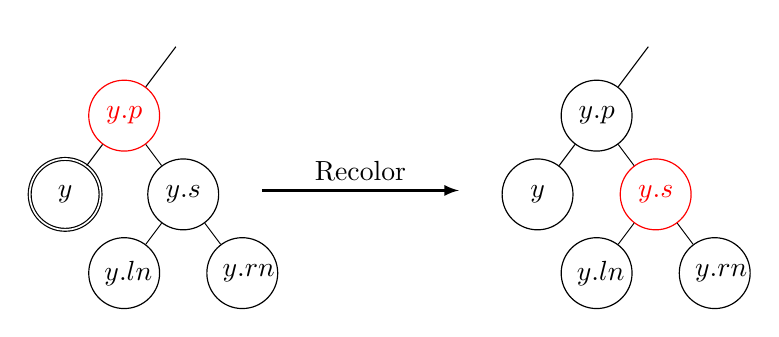
\begin{tikzpicture}[level distance=1cm,
				      every node/.style={align=center, line width=0.15mm},
				      level 1/.style={sibling distance=1.5cm},
				      level 2/.style={sibling distance=1.5cm},
				      redVertex/.style={
						      draw, shape=circle,
						      minimum width=0.9cm, minimum height=0.5cm,
						      inner sep=0pt, text width=0.5cm, text centered,
						      text=red!75!black, color=red
					      },
				      blackVertex/.style={
						      draw, shape=circle,
						      minimum width=0.9cm, minimum height=0.5cm,
						      inner sep=0pt, text width=0.5cm, text centered
					      },
				      doubleBlackVertex/.style={
						      draw, double, shape=circle,
						      minimum width=0.9cm, minimum height=0.5cm,
						      inner sep=0pt, text width=0.5cm, text centered
					      },
				      every edge/.style = {draw, latex'-latex', line width=0.3mm, dotted},
				      parentarrow/.style={line width=0.12mm}
			      ]

			      % Leftmost tree
			      \node (AA0) {}
			      child{
					      node[redVertex] (A2) {$y.p$}
					      child {node[doubleBlackVertex] (B2) {$y$}}
					      child {
							      node[blackVertex] (C2) {$y.s$} edge from parent[parentarrow]
							      child {node[blackVertex] (D2) {$y.ln$} edge from parent[parentarrow]}
							      child {node[blackVertex] (E2) {$y.rn$} }
							      edge from parent[parentarrow]
						      }
				      }
			      child [missing] { node (AA5) {} };
			      % Right tree
			      \begin{scope}[shift={(6,0)}]
				      \node (A0) {}
				      child{
						      node[blackVertex] (A1) {$y.p$}
						      child {node[blackVertex] (B1) {$y$}}
						      child {
								      node[redVertex] (C1) {$y.s$} edge from parent[parentarrow]
								      child {node[blackVertex] (D1) {$y.ln$} edge from parent[parentarrow]}
								      child {node[blackVertex] (E1) {$y.rn$} }
								      edge from parent[parentarrow]
							      }
					      }
				      child [missing] { node (A5) {} };
			      \end{scope}

			      \draw[thick, -latex] ($(C2)+(1,0.05)$) -- node[midway, above] {Recolor} ($(B1)+(-1,0.05)$);
		      \end{tikzpicture}
	      \end{figure}
	\item $y.\emph{sibling}$ is Black and $y.\emph{right-nephew}$ is Red. Then we do a \textsc{Left-Rotate} on $y.\emph{parent}$. And we recolor
	      \begin{figure}[!h]
		      \centering
		      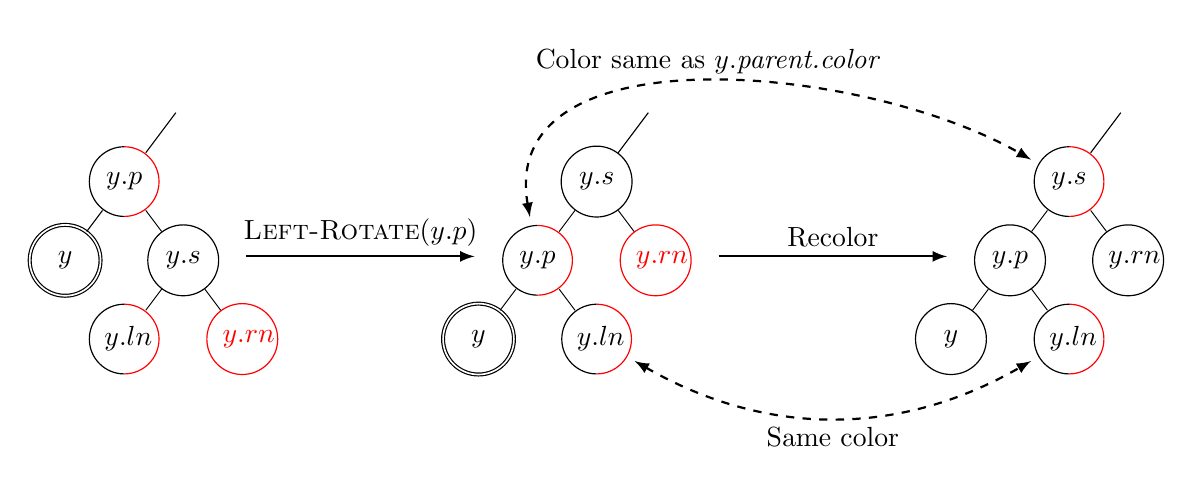
\begin{tikzpicture}[level distance=1cm, sibling distance=1.5cm,
				      every node/.style={align=center, line width=0.15mm},
				      redVertex/.style={
						      draw, shape=circle,
						      minimum width=0.9cm, minimum height=0.5cm,
						      inner sep=0pt, text width=0.5cm, text centered,
						      text=red!75!black, color=red
					      },
				      blackVertex/.style={
						      draw, shape=circle,
						      minimum width=0.9cm, minimum height=0.5cm,
						      inner sep=0pt, text width=0.5cm, text centered
					      },
				      doubleBlackVertex/.style={
						      draw, double, shape=circle,
						      minimum width=0.9cm, minimum height=0.5cm,
						      inner sep=0pt, text width=0.5cm, text centered
					      },
				      halfBorderVertex/.style={
						      circle,
						      minimum width=0.9cm,
						      inner sep=0pt,
						      text width=0.5cm,
						      text centered,
						      path picture={
								      \draw[black, line width=0.3mm]
								      (path picture bounding box.center) ++(90:0.45cm) arc[start angle=90, end angle=270, radius=0.45cm];
								      \draw[red, line width=0.3mm]
								      (path picture bounding box.center) ++(270:0.45cm) arc[start angle=270, end angle=450, radius=0.45cm];
							      }
					      },
				      parentarrow/.style={line width=0.12mm}
			      ]

			      % Leftmost tree
			      \node (AA0) {}
			      child{
					      node[halfBorderVertex] (A2) {$y.p$}
					      child {node[doubleBlackVertex] (B2) {$y$}}
					      child {
							      node[blackVertex] (C2) {$y.s$} edge from parent[parentarrow]
							      child {node[halfBorderVertex] (D2) {$y.ln$} edge from parent[parentarrow]}
							      child {node[redVertex] (E2) {$y.rn$} }
							      edge from parent[parentarrow]
						      }
				      }
			      child [missing] { node (AA5) {} };
			      % Right tree
			      \begin{scope}[shift={(6,0)}]
				      \node (A0) {}
				      child{
						      node[blackVertex] (A1) {$y.s$}
						      child {
								      node[halfBorderVertex] (B1) {$y.p$}
								      child {node[doubleBlackVertex] (D1) {$y$} edge from parent[parentarrow]}
								      child {node[halfBorderVertex] (E1) {$y.ln$} }
								      edge from parent[parentarrow]
							      }
						      child {node[redVertex] (C1) {$y.rn$} edge from parent[parentarrow]}
					      }
				      child [missing] { node (A5) {} };
			      \end{scope}

			      \begin{scope}[shift={(12,0)}]
				      \node (AAA0) {}
				      child{
						      node[halfBorderVertex] (A3) {$y.s$}
						      child {
								      node[blackVertex] (B3) {$y.p$}
								      child {node[blackVertex] (D3) {$y$} edge from parent[parentarrow]}
								      child {node[halfBorderVertex] (E3) {$y.ln$} }
								      edge from parent[parentarrow]
							      }
						      child {node[blackVertex] (C3) {$y.rn$} edge from parent[parentarrow]}
					      }
				      child [missing] { node (AAA5) {} };
			      \end{scope}

			      \draw[thick, -latex] ($(C2)+(0.8,0.05)$) -- node[midway, above] {\textsc{Left-Rotate}$(y.p)$} ($(B1)+(-0.8,0.05)$);
			      \draw[thick, -latex] ($(C1)+(0.8,0.05)$) -- node[midway, above] {Recolor} ($(B3)+(-0.8,0.05)$);
			      \draw[thick, dashed,latex-latex] (E1) edge [bend right=30, shorten <=1mm, shorten >=1mm] node[midway, below] {Same color} (E3);
			      \draw[thick, dashed, latex-latex]
			      (B1) edge [
					      out=100,          % angle leaving B1
					      in=150,          % angle entering E3
					      looseness=1,   % (optional) controls curvature
					      shorten <=1mm,
					      shorten >=1mm
				      ]
			      node[midway, above] {Color same as $y.\emph{parent.color}$}
			      (A3);
		      \end{tikzpicture}
	      \end{figure}  $y.\emph{parent}$ to black and $y.\emph{right-nephew}$ to red and $y$ to black. We color $y.\emph{sibling}$ to the same color as $y.\emph{parent}$. And now we stop.
	\item $y.\emph{sibling},y.\emph{right-nephew}$ are Black \& $y.\emph{left-nephew}$ is Red. Therefore, both the children of $y.\emph{left-nephew}$ have color black. Here we first do a \textsc{Right-Rotate} on $y.\emph{sibling}$.
	      \begin{figure}[!h]
		      \centering
		      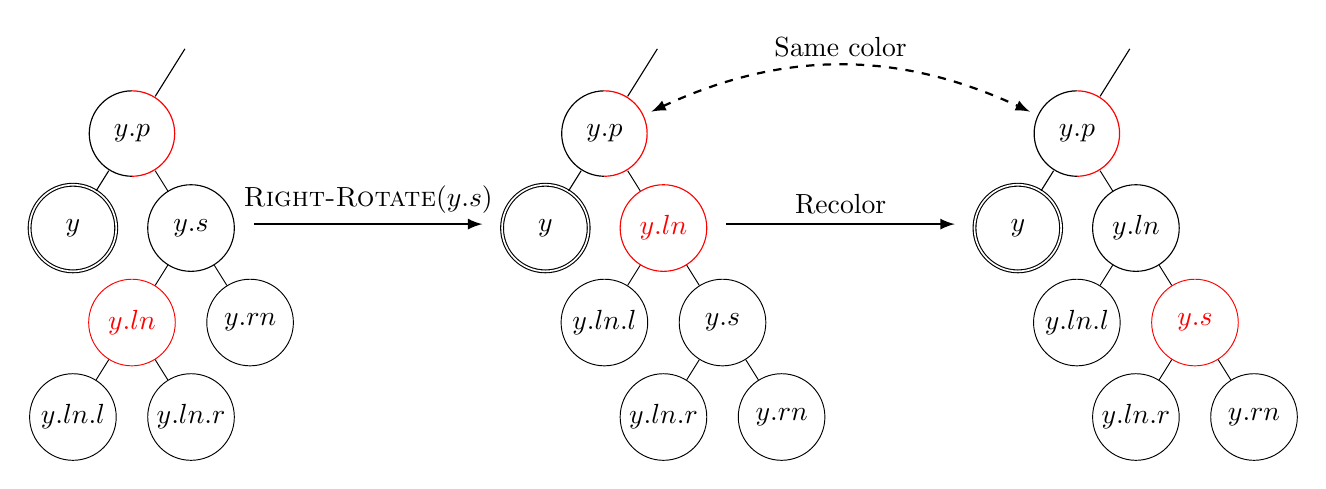
\begin{tikzpicture}[level distance=1.2cm, sibling distance=1.5cm,
				      redVertex/.style={
						      draw, shape=circle,
						      minimum width=1.1cm, minimum height=0.5cm,
						      inner sep=0pt, text width=1cm, text centered,
						      text=red!75!black, color=red
					      },
				      blackVertex/.style={
						      draw, shape=circle,
						      minimum width=1.1cm, minimum height=0.5cm,
						      inner sep=0pt, text width=1cm, text centered
					      },
				      doubleBlackVertex/.style={
						      draw, double, shape=circle,
						      minimum width=1.1cm, minimum height=0.5cm,
						      inner sep=0pt, text width=1cm, text centered
					      },
				      halfBorderVertex/.style={
						      circle,
						      minimum width=1.1cm,
						      inner sep=0pt,
						      text width=1cm,
						      text centered,
						      path picture={
								      \draw[black, line width=0.3mm]
								      (path picture bounding box.center) ++(90:0.55cm) arc[start angle=90, end angle=270, radius=0.55cm];
								      \draw[red, line width=0.3mm]
								      (path picture bounding box.center) ++(270:0.55cm) arc[start angle=270, end angle=450, radius=0.55cm];
							      }
					      },
				      parentarrow/.style={line width=0.12mm}
			      ]

			      % Leftmost tree
			      \node (AA0) {}
			      child{
					      node[halfBorderVertex] (A2) {$y.p$}
					      child {node[doubleBlackVertex] (B2) {$y$}}
					      child {
							      node[blackVertex] (C2) {$y.s$} edge from parent[parentarrow]
							      child {
									      node[redVertex] (D2) {$y.ln$} edge from parent[parentarrow]
									      child { node[blackVertex] (F2) {$y.ln.l$} }
									      child { node[blackVertex] (G2) {$y.ln.r$} }
								      }
							      child {node[blackVertex] (E2) {$y.rn$} }
							      edge from parent[parentarrow]
						      }
				      }
			      child [missing] { node (AA5) {} };
			      % Right tree
			      \begin{scope}[shift={(6,0)}]
				      \node (A0) {}
				      child{
						      node[halfBorderVertex] (A1) {$y.p$}
						      child {node[doubleBlackVertex] (B1) {$y$}}
						      child {
								      node[redVertex] (C1) {$y.ln$} edge from parent[parentarrow]
								      child {										      node[blackVertex] (D1) {$y.ln.l$} edge from parent[parentarrow]									      }
								      child {
										      node[blackVertex] (E1) {$y.s$}
										      child { node[blackVertex] (F1) {$y.ln.r$} }
										      child { node[blackVertex] (G1) {$y.rn$} }
									      }
								      edge from parent[parentarrow]
							      }
					      }
				      child [missing] { node (A5) {} };
			      \end{scope}

			      \begin{scope}[shift={(12,0)}]
				      \node (AAA0) {}
				      child{
						      node[halfBorderVertex] (A3) {$y.p$}
						      child {node[doubleBlackVertex] (B3) {$y$}}
						      child {
								      node[blackVertex] (C3) {$y.ln$} edge from parent[parentarrow]
								      child {										      node[blackVertex] (D3) {$y.ln.l$} edge from parent[parentarrow]									      }
								      child {
										      node[redVertex] (E3) {$y.s$}
										      child { node[blackVertex] (F3) {$y.ln.r$} }
										      child { node[blackVertex] (G3) {$y.rn$} }
									      }
								      edge from parent[parentarrow]
							      }
					      }
				      child [missing] { node (AAA5) {} };
			      \end{scope}

			      \draw[thick, -latex] ($(C2)+(0.8,0.05)$) -- node[midway, above] {\textsc{Right-Rotate}$(y.s)$} ($(B1)+(-0.8,0.05)$);
			      \draw[thick, -latex] ($(C1)+(0.8,0.05)$) -- node[midway, above] {Recolor} ($(B3)+(-0.8,0.05)$);
			      \draw[thick, dashed,latex-latex] (A1) edge [bend left=25, shorten <=1mm, shorten >=1mm] node[midway, above] {Same color} (A3);
		      \end{tikzpicture}
	      \end{figure}Then we recolor $y.\emph{left-nephew}$ to black and $y.\emph{sibling}$ to red. Now we have exactly the same situation as in Case III. So we follow the steps of Case III.
	\item $y.\emph{sibling}=$ Red. In this case $y.\emph{left-newphew}$ and $y.\emph{right-nephew}$ must be black. Then we do a \textsc{Left-Rotate} on $y.\emph{parent}$.
	      \begin{figure}[!h]
		      \centering
		      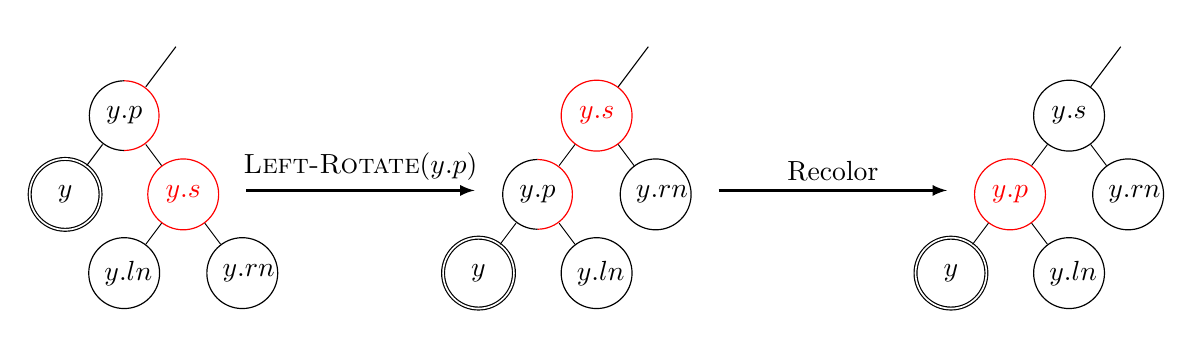
\begin{tikzpicture}[level distance=1cm, sibling distance=1.5cm,
				      every node/.style={align=center, line width=0.15mm},
				      redVertex/.style={
						      draw, shape=circle,
						      minimum width=0.9cm, minimum height=0.5cm,
						      inner sep=0pt, text width=0.5cm, text centered,
						      text=red!75!black, color=red
					      },
				      blackVertex/.style={
						      draw, shape=circle,
						      minimum width=0.9cm, minimum height=0.5cm,
						      inner sep=0pt, text width=0.5cm, text centered
					      },
				      doubleBlackVertex/.style={
						      draw, double, shape=circle,
						      minimum width=0.9cm, minimum height=0.5cm,
						      inner sep=0pt, text width=0.5cm, text centered
					      },
				      halfBorderVertex/.style={
						      circle,
						      minimum width=0.9cm,
						      inner sep=0pt,
						      text width=0.5cm,
						      text centered,
						      path picture={
								      \draw[black, line width=0.3mm]
								      (path picture bounding box.center) ++(90:0.45cm) arc[start angle=90, end angle=270, radius=0.45cm];
								      \draw[red, line width=0.3mm]
								      (path picture bounding box.center) ++(270:0.45cm) arc[start angle=270, end angle=450, radius=0.45cm];
							      }
					      },
				      parentarrow/.style={line width=0.12mm}
			      ]

			      % Leftmost tree
			      \node (AA0) {}
			      child{
					      node[halfBorderVertex] (A2) {$y.p$}
					      child {node[doubleBlackVertex] (B2) {$y$}}
					      child {
							      node[redVertex] (C2) {$y.s$} edge from parent[parentarrow]
							      child {node[blackVertex] (D2) {$y.ln$} edge from parent[parentarrow]}
							      child {node[blackVertex] (E2) {$y.rn$} }
							      edge from parent[parentarrow]
						      }
				      }
			      child [missing] { node (AA5) {} };
			      % Right tree
			      \begin{scope}[shift={(6,0)}]
				      \node (A0) {}
				      child{
						      node[redVertex] (A1) {$y.s$}
						      child {
								      node[halfBorderVertex] (B1) {$y.p$}
								      child {node[doubleBlackVertex] (D1) {$y$} edge from parent[parentarrow]}
								      child {node[blackVertex] (E1) {$y.ln$} }
								      edge from parent[parentarrow]
							      }
						      child {node[blackVertex] (C1) {$y.rn$} edge from parent[parentarrow]}
					      }
				      child [missing] { node (A5) {} };
			      \end{scope}

			      \begin{scope}[shift={(12,0)}]
				      \node (AAA0) {}
				      child{
						      node[blackVertex] (A3) {$y.s$}
						      child {
								      node[redVertex] (B3) {$y.p$}
								      child {node[doubleBlackVertex] (D3) {$y$} edge from parent[parentarrow]}
								      child {node[blackVertex] (E3) {$y.ln$} }
								      edge from parent[parentarrow]
							      }
						      child {node[blackVertex] (C3) {$y.rn$} edge from parent[parentarrow]}
					      }
				      child [missing] { node (AAA5) {} };
			      \end{scope}

			      \draw[thick, -latex] ($(C2)+(0.8,0.05)$) -- node[midway, above] {\textsc{Left-Rotate}$(y.p)$} ($(B1)+(-0.8,0.05)$);
			      \draw[thick, -latex] ($(C1)+(0.8,0.05)$) -- node[midway, above] {Recolor} ($(B3)+(-0.8,0.05)$);
		      \end{tikzpicture}
	      \end{figure}Then we recolor $y.\emph{parent}$ to black and $y.\emph{sibling}$ to red. Now we have the sibling of $y$ has color black. So we are now in one of the previous cases. So we can follow the suitable case to resolve.
\end{enumerate}
This completes the description of the deletion process in a red-black tree. Now notice every time we are pushing the double-black color up the tree, or we are stopping. Hence, it only takes $O(\log n)$ time to resolve the double-black color. So the deletion process in a red-black tree takes $O(\log n)$ time.